\documentclass[a4paper,12pt]{report}
\usepackage{alltt, fancyvrb, url}
\usepackage{graphicx}
\usepackage[utf8]{inputenc}
\usepackage{float}
\usepackage{hyperref}
\usepackage{minted}
\usepackage{tcolorbox}
\usepackage{booktabs}

\newcommand{\myexample}[2]{
    \begin{tcolorbox}[colback=black!5!white,colframe=black,title={Esempio: #1}]
        #2
    \end{tcolorbox}
}
\graphicspath{{./images}}

% Questo commentalo se vuoi scrivere in inglese.
\usepackage[italian]{babel}

\usepackage[italian]{cleveref}
\title{Relazione del progetto di Programmazione di Reti 
    \\ Traccia 1: Configurazione di una Rete con VLAN e Routing Inter-VLAN}

\author{Leonardo Grimaldi}
\date{\today}   
\begin{document}
\maketitle
\tableofcontents
\chapter{Consegna}
\section{Descrizione}
Gli studenti dovranno progettare e configurare una rete che include due LAN separate in due VLAN su Cisco Packet Tracer, utilizzando switch e router virtuali. La configurazione richiederà il routing inter-VLAN per permettere la comunicazione tra le VLAN.
\section{Obiettivi}
Configurare VLAN, routing inter-VLAN, e verificare la connettività tra dispositivi su VLAN diverse.
\section{Consegne richieste}
Documentazione della configurazione, spiegazione dei comandi utilizzati e cattura del traffico di rete per dimostrare la comunicazione tra le VLAN.
\chapter{Progettazione}
\label{chap:progettazione}
I due campus dell'Università di Bologna, il Campus di Cesena e il Campus di Bologna sono costituiti da due dipartimenti: IT (Information Technology) e di ricerca.
%
Essi possiedono due edge router che possono scambiarsi informazioni per mezzo di una WAN (Wide Area Network), semplificato con un collegamento diretto.
%
Il traffico dei dipartimenti all'interno del singolo Campus vuole essere separato, mentre si vuole consentire la comunicazione inter-dipartimentale tra i due Campus.
%
\myexample{Ping tra i Campus}{
    Scientifico Cesena Scientifico Bologna
    %
    Scientifico Cesena  IT Bologna
}
La topologia di rete è proposta nella figura \ref{fig:topologia_offline}. 
\begin{figure}
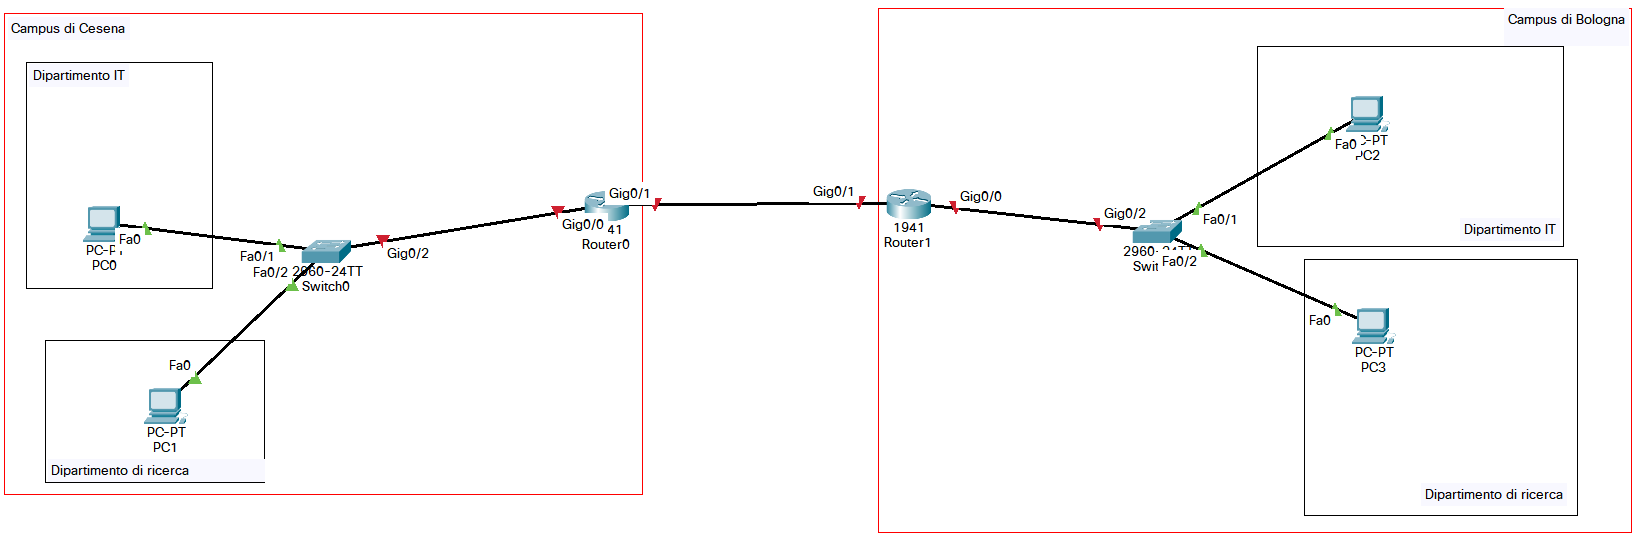
\includegraphics[width=\textwidth]{offline_topology_with_departments.png}
\caption{
    Topologia di rete dei dipartimenti di IT e ricerca tra il Campus di Cesena e Bologna.
    %
    I triangolini rossi sui collegamenti indicano che il link è offline.
    }
\label{fig:topologia_offline}
\end{figure}
\chapter{Configurazione}
Si assume che tutti i dispositivi siano accesi e le configurazioni siano effettuate tramite il terminale del dispositivo scelto.
%
Nel caso dei Personal Computer verrà utilizzata l'interfaccia grafica di Cisco Packet Tracer, pur sapendo che nel mondo reale i computer hanno un sistema operativo e le proprie modalità di configurazione.
%
\\Si nota inoltre che ogni comando Cisco si può abbreviare e nelle successive schermate \mintinline{text}|configure terminal|, come altri comandi, potrebbe diventare \mintinline{text}|conf t|.
%
Qualora il lettore non conoscesse la keyword completa del comando, si raccomanda di scrivere il comando abbreviato e premere il tasto \texttt{Tab} per mostrare la forma completa.
%
In ogni caso, si può sempre far riferimento al manuale utilizzando il comando \texttt{?}, oppure consultare un \href{https://www.websentra.com/cisco-commands-cheat-sheet/}{cheat sheet} online.
%
\\È altresì importante ricordare che i comandi dei dispositivi Cisco fisici non coincidono necessariamente con quelli di Cisco Packet Tracer.
%
Sarà cura del lettore documentarsi e trovare il comando corrispondente.
\section{Pianificazione}
Innanzitutto, è necessario stabilire gli indirizzi IP per i computer e per le interfacce dei router.
\begin{table}[]
\begin{tabular}{@{}lllll@{}}
\toprule
Dispositivo & Interfaccia & Indirizzo IP & Subnet & Gateway \\ \midrule
Router0 & Gig0/0 & 10.0.0.1 & 255.255.255.0 & 10.0.0.1 \\
Router0 & Gig0/1 & 13.0.0.1 & 255.255.255.252 & N/A \\
PC0 & Fa0 & 10.0.1.2 & 255.255.255.0 & 10.0.1.1 \\
PC1 & Fa0 & 10.0.2.2 & 255.255.255.0 & 10.0.2.1 \\ \bottomrule
\end{tabular}
\caption{Configurazione rete Campus di Cesena}
\label{table:config_cesena}
\end{table}
\begin{table}[]
\begin{tabular}{lllll}
\hline
Dispositivo & Interfaccia & Indirizzo IP & Subnet & Gateway \\ \hline
Router1 & Gig0/0.30 & 13.0.3.1 & 255.255.255.0 & 13.0.3.1 \\
Router1 & Gig0/0.40 & 13.0.4.1 & 255.255.255.0 & 13.0.4.1 \\
PC3 & Fa0 & 13.0.3.2 & 255.255.255.0 & 13.0.3.1 \\
PC4 & Fa0 & 13.0.4.2 & 255.255.255.0 & 13.0.4.1 \\ \hline
\end{tabular}
\caption{Configurazione rete Campus di Bologna}
\label{table:config_bologna}
\end{table}
\begin{table}[]
\begin{tabular}{@{}lllll@{}}
\toprule
Dispositivo & Campus & Dipartimento & VLAN & Nome VLAN \\ \midrule
PC1 & Cesena & IT & 10 & IT\_Cesena \\
PC2 & Cesena & Ricerca & 20 & Ricerca\_Cesena \\
PC3 & Bologna & IT & 30 & IT\_Bologna \\
PC4 & Bologna & Ricerca & 40 & Ricerca\_Bologna \\ \bottomrule
\end{tabular}
\caption{Ripartizione delle VLAN}
\label{table:vlan_division}
\end{table}
\section{Switch}
Inizialmente si configura lo switch della rete interna.
%
In questa sezione verrà usato come esempio lo \texttt{Switch0}, ma il procedimento sarà analogo anche per lo Switch1 nella rete di Bologna, facendo riferimento alla tabella \ref{table:vlan_division} per le VLAN da assegnare.
Il primo step di configurazione del dispositivo è assegnargli il nome giusto.
%
Si entra in modalità privilegiata con il comando \mintinline{text}|enable| e nella configurazione del terminale (accessibile solo dalla modalità privilegiata) con \mintinline{text}|configure terminal|.
\begin{minted}[]{text}
Switch>
Switch>enable
Switch#config terminal
Enter configuration commands, one per line.  End with CNTL/Z.
Switch(config)#hostname Switch0
Switch0#
\end{minted}
Il comando \texttt{hostname <nome>} ha consentito di assegnare un nuovo nome allo switch.
\\Terminiamo questo primo passaggio di configurazione salvando i cambiamenti.
\begin{minted}[]{text}
Switch0(config)#exit
Switch0#
%SYS-5-CONFIG_I: Configured from console by console
Switch0#copy ru st
Destination filename [startup-config]? 
Building configuration...
[OK]
Switch0#
\end{minted}
Come procedura operativa standard, ci assicureremo sempre di salvare la configurazione dopo ogni cambiamento importante. 
\subsection{Creazione VLAN}
\begin{figure}
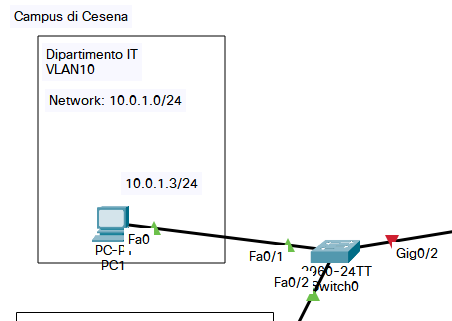
\includegraphics[]{configurazione_switch.png}
\caption{Switch interno della rete del campus di Cesena}
\label{fig:switch_cesena}
\end{figure}
\begin{minted}{text}
Switch0(config)#vlan 10
Switch0(config-vlan)#
%LINK-5-CHANGED: Interface Vlan10, changed state to up

Switch0(config-vlan)#name IT_Cesena
Switch0(config-vlan)#vlan 20
Switch0(config-vlan)#name Ricerca_Cesena
Switch0(config-vlan)#
\end{minted}
Abbiamo creato la VLAN 10 e la VLAN 20 e assegnatoli il nome secondo la tabella \ref{table:vlan_division}
In modalità privilegiata possiamo vedere che sono state aggiunte.
\begin{minted}{text}
Switch0# show vlan brief
VLAN Name                             Status    Ports
---- -------------------------------- --------- -------------------------------
1    default                          active    Fa0/1, Fa0/2, Fa0/3, Fa0/4
                                                Fa0/5, Fa0/6, Fa0/7, Fa0/8
                                                Fa0/9, Fa0/10, Fa0/11, Fa0/12
                                                Fa0/13, Fa0/14, Fa0/15, Fa0/16
                                                Fa0/17, Fa0/18, Fa0/19, Fa0/20
                                                Fa0/21, Fa0/22, Fa0/23, Fa0/24
                                                Gig0/1, Gig0/2
10   IT_Cesena                        active    
20   Ricerca_Cesena                   active    
1002 fddi-default                     active    
1003 token-ring-default               active    
1004 fddinet-default                  active    
1005 trnet-default                    active    
Switch0# copy ru st
\end{minted}
\subsection{Assegnazione porte alle VLAN}
Per le interfacce collegate ai singoli dipartimenti sarà necessario usare la modalità \textbf{access} per dire allo switch che su quel link scorre esclusivamente traffico di una singola VLAN.
%
Inoltre, si dovrà assegnare l'interfaccia alla VLAN adeguata.
\begin{minted}{text}
Switch0(config)#int vlan 10
Switch0(config-if)#ip addr 10.0.1.2 255.255.255.0
Switch0(config)#int Fa0/1
Switch0(config-if)#switchport mode access
Switch0(config-if)#switchport access vlan 10
Switch0(config-if)#
%LINEPROTO-5-UPDOWN: Line protocol on Interface Vlan10, changed state to up
Switch0(config-if)#
\end{minted} 
In questo modo è stata completata la parte del dipartimento IT.
%
Analogamente, si eseguono gli stessi passi per l'interfaccia legata al dipartimento di ricerca.
\subsection{Assegnazione porta trunk}
Il traffico delle due VLAN dovrà attraversare canale fisico comune collegato alla interfaccia Gig0/2.
%
Per questo, dovremo porre una regola sull'utilizzo di quella interfaccia e dire allo Switch che essa viene attraversata da molteplici VLAN (nel nostro caso due).
%
Questo tipo di regola si chiama \textbf{trunking} e basterà un semplice comando per attivarla.
\begin{minted}{text}
Switch0(config)#int Gig0/2
Switch0(config-if)#switchport mode trunk
Switch0(config-if)#exit
Switch0(config)#exit
Switch0# copy ru st
\end{minted}
\section{PC}
Questa parte di configurazione è la più breve e semplice; basta assegnare i giusti indirizzi IP, gateway e subnet mask ai computer facendo riferimento alla tabella \ref{table:config_cesena} per la rete di Cesena e \ref{table:config_bologna} per la rete di Bologna.
%
Come accennato a inizio capitolo, verrà usata la interfaccia grafica di Cisco, ma nel mondo reale i PC avranno un loro sistema operativo dal quale si potrà assegnare l'IP, o ancora meglio, nella rete vi sarà un server DHCP che automatizza il processo.
%
Di seguito è riportato un estratto della configurazione statica del PC1 nella rete di Cesena.
\begin{figure}
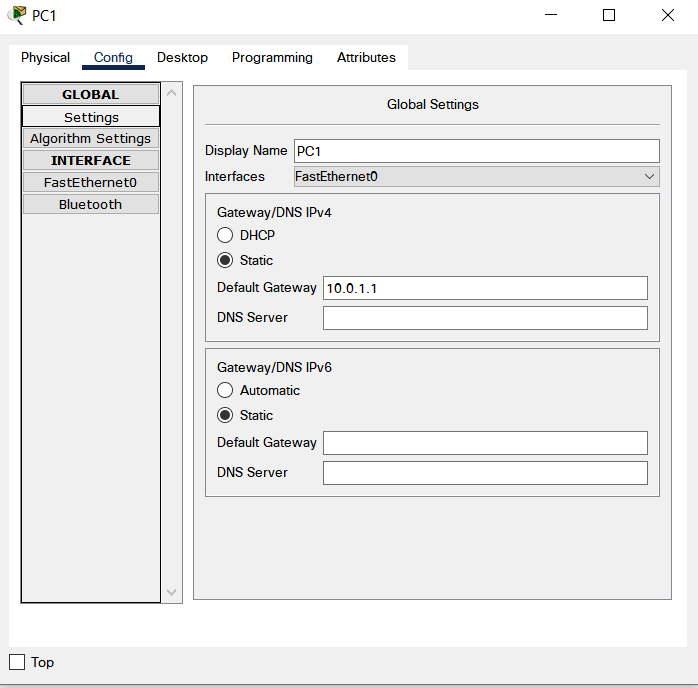
\includegraphics[]{pc1_gateway_config.png}
\caption{Configurazione gateway PC1}
\label{fig:pc1_gateway_config}
\end{figure}
\begin{figure}
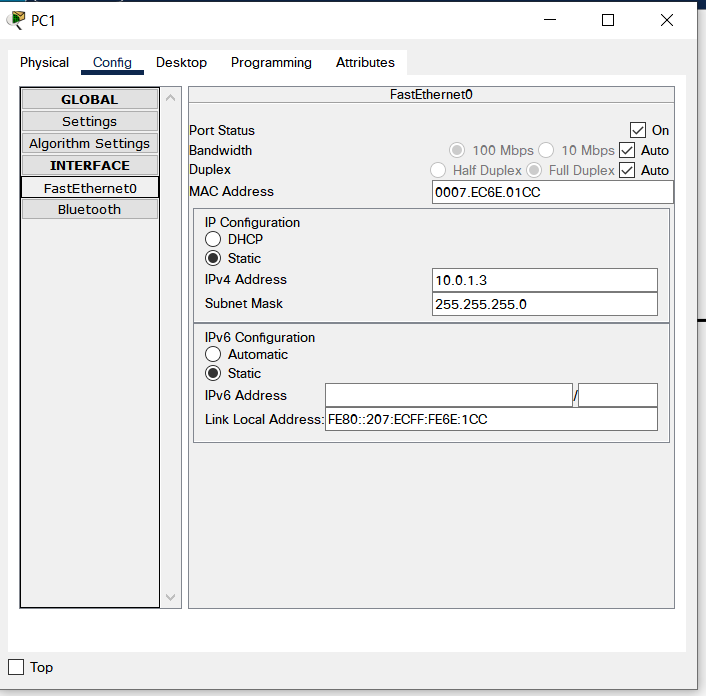
\includegraphics[]{pc1_ip_config.png}
\caption{Configurazione IP PC1}
\label{fig:pc1_ip_config}
\end{figure}
\subsection{Test di comunicazione tra PC1 e PC2}
Una prova più profonda sarà eseguita nel capitolo \nameref{chap:testing}, ma per configurare una rete grossa è molto importante proseguire incrementalmente ed eseguire vari test per assicurarsi che il lavoro fatto finora sia funzionante.
In questa sezione si esegue la verifica tra PC1 e PC2, ma è consigliabile farla anche su PC3 e PC4 (o tutti i dispositivi finora configurati).
Proseguendo, ci si aspetta che la comunicazione tra la VLAN 10 e VLAN 20 non sia possibile per due motivi:
\begin{enumerate}
    \item I due dipartimenti sono su reti diverse
    \item Le due reti appartengono a VLAN differenti, che non hanno un routing inter-VLAN
\end{enumerate}
Ovviamente questo sarebbe il comportamento corretto rispetto alle specifiche del capitolo \nameref{chap:progettazione}, dato che i due dipartimenti differenti non possono comunicare.
%
Per eseguire il test si apre il terminale del PC1 e si esegue un ping verso l'IP \texttt{10.0.2.3}
\begin{figure}
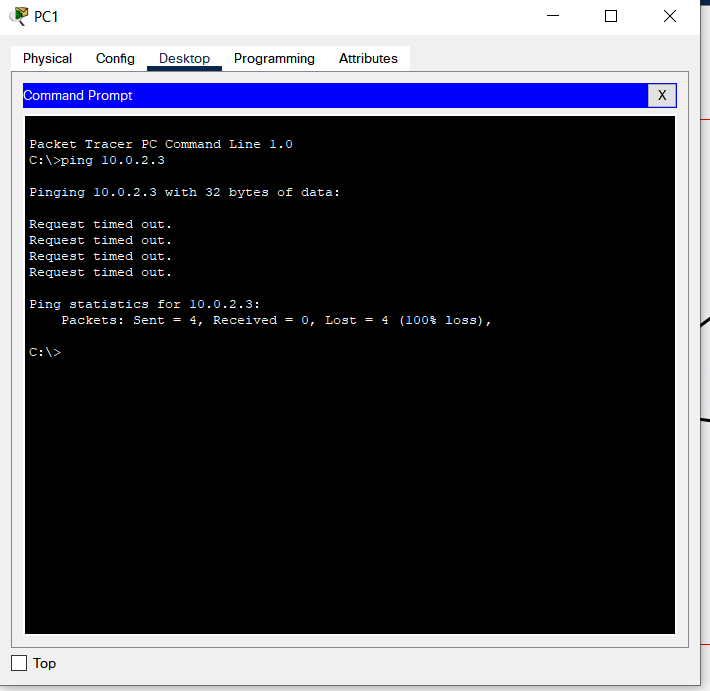
\includegraphics[]{pc1_test_vlan_differenti.png}
\caption{Esecuzione ping 10.0.2.3 sul PC1 con conseguente fallimento}
\label{fig:pc1_test_vlan_differenti}
\end{figure}
Come si può vedere dalla figura \ref{fig:pc1_test_vlan_differenti} il ping non è andato a buon fine.
\section{Router}
La parte finale è più complessa prevede la configurazione dei due edge router delle nostre reti.
%
Prima di tutto, si dovranno configurare le interfacce interne (quelle collegate allo switch), in modo da consentire i pacchetti dei PC di passare attraverso il trunk: $$switch \longleftrightarrow router$$
%
Successivamente, si configureranno le interfacce esterne dei Router0 e Router1 per poter farli comunicare.
%
Solo quando questi processi risulteranno andati a buon fine si potrà configurare la comuncazione tra i dipartimenti intra-campus.
\subsection{Configurazione trunk porta interna (Gig0/0)}
Sull'interfaccia Gig0/0 del Router0 passa il traffico VLAN10 e VLAN20 ed e quindi necessario creare delle sottointerfacce virtuali che gestiscano questo traffico.
%
In partenza si accende l'interfaccia Gig0/0 con \texttt{no shut} e poi si configurano le \textit{sub interfaces} Gig0/0.10 e Gig/0.20 (come da tabella \ref{table:config_cesena}).
%
Si usa il comando \texttt{encapsulation dot1q \textit{numero\_vlan}} per dire al router di usare il tagging VLAN e abilitare il routing delle VLAN.
\begin{minted}{text}
Router0(config)#int Gig0/0
Router0(config-if)#no shut

Router0(config-if)#
%LINK-5-CHANGED: Interface GigabitEthernet0/0, changed state to up

%LINEPROTO-5-UPDOWN: Line protocol on Interface GigabitEthernet0/0, changed state to up

Router0(config-if)#int Gig0/0.10
Router0(config-subif)#
%LINK-5-CHANGED: Interface GigabitEthernet0/0.10, changed state to up

%LINEPROTO-5-UPDOWN: Line protocol on Interface GigabitEthernet0/0.10, changed state to up

Router0(config-subif)#encapsulation dot1q 10
Router0(config-subif)#ip add 10.0.1.1 255.255.255.0
Router0(config-subif)#no shut
Router0(config-subif)#int Gig0/0.20
Router0(config-subif)#
%LINK-5-CHANGED: Interface GigabitEthernet0/0.20, changed state to up

%LINEPROTO-5-UPDOWN: Line protocol on Interface GigabitEthernet0/0.20, changed state to up
ip add 10.0.2.1 255.255.255.0

% Configuring IP routing on a LAN subinterface is only allowed if that
subinterface is already configured as part of an IEEE 802.10, IEEE 802.1Q,
or ISL vLAN.

Router0(config-subif)#encapsulation dot1q 20
Router0(config-subif)#ip add 10.0.2.1 255.255.255.0
Router0(config-subif)#no shut
Router0(config-subif)#
\end{minted}
Ora i due computer possono raggiungere il router, ma abbiamo creato un nuovo problema: \texttt{le due VLAN riescono a parlarsi}
\subsection{Disabilitare il routing inter-VLAN}
\subsection{Abilitare la comunicazione tra Router0 e Router1}
Questa parte è molto semplice: basta seguire la tabella \ref{table:config_cesena} e \ref{table:config_bologna} per assegnare gli ip alle interfacce.
Di seguito la configurazione del Router0:
\begin{minted}{text}
Router0(config)#int Gig0/1
Router0(config-if)#ip addr 22.0.0.1 255.255.255.252
Router0(config-if)#no shut
\end{minted}
Successivamente, la configurazione del Router1:
\begin{minted}{text}
Router1(config)#int Gig0/1
Router1(config-if)#ip addr 22.0.0.2 255.255.255.252
Router1(config-if)#no shut
\end{minted}
\subsection{Assegnare le rotte statiche per abilitare la  comunicazione tra gli stessi dipartimenti}
\begin{minted}{text}
Router0(config)#ip route 13.0.3.0 255.255.255.0 22.0.0.2
Router0(config)#ip route 13.0.4.0 255.255.255.0 22.0.0.2
\end{minted}
\begin{minted}{text}
Router1(config)#ip route 10.0.1.0 255.255.255.0 22.0.0.1
Router1(config)#ip route 10.0.2.0 255.255.255.0 22.0.0.1
\end{minted}
\chapter{Testing}
\label{chap:testing}
\section{Riferimenti}
https://computernetworking747640215.wordpress.com/2018/07/05/vlan-configuration-on-a-cisco-switch-in-packet-tracer/
%
% https://networklessons.com/switching/intervlan-routing#SVI_Switch_Virtual_Interface
% https://www.practicalnetworking.net/stand-alone/routing-between-vlans/
\end{document}